% ------------------------- MAIN TASK ---------------------------------
\section{Reprise du projet}
\paragraph{Le projet à été repris d'un ancien collègue, dont le cahier des charges initial était :}

Concevoir un système pouvant reconnaitre des formes simples à l’aide d’une caméra, et de la librairie OpenCV, et de pouvoir implémenter cela sur un Raspberry Pi.

\subsection{État initial du projet repris}
\paragraph{La version finale du projet repris était :} Forme non-achevée du code permettant de reconnaître des formes simples. Cependant, début de travail.

\subsection{Méthode et objectifs de la reprise}
L'objectif final du projet est d'avoir un code capable de dessiner les contours des formes.
La prochaine étape de ce projet consistera à finaliser le code de reconnaissance des formes simples. Ce code sera capable de reconnaître des formes telles qu'un cercle, un carré ou un triangle, et d'afficher leurs noms soit sur une interface graphique, soit dans une console.
Une fois que ce code sera développé, veuillez vous référer au cahier des charges (voir annexe) pour le reste des tâches de ce projet.

Pour la suite du projet, j'ai décidé de choisi le langage Python, car elle permet une approche plus simple de ce genre d'algorithme et est plus facilement implémentable sur raspberry.

\paragraph{Objectifs :}
Mon objectif est dans un premier temps de faire fonctionner le code de reconnaissance d'image avec des formes simples issues d'une base de donnée, puis de l'étendre pour des images plus complexes et réelles.


%---
\clearpage
\section{Programmation Python}
A des fins de simplification, j'ai décidé d'utiliser la distribution python Anaconda, qui permet de plus simplement gérer les paquets afin de mieux traiter les différentes dépendances, concurrent direct de pip.

\subsection{Implémentation OpenCV}
La librairie de python-opencv n'est qu'une enveloppe autour du code C/C++ original. Il est normalement utilisé pour combiner les meilleures caractéristiques des deux langages, la performance de C/C++ et la simplicité de Python.

\paragraph{Installation d'open-cv :}
\begin{verbatim}
	conda install -c conda-forge opencv
\end{verbatim}
En plus de ce package, j'utiliserais d'autres tels que numpy, matplotlib etc... (Voir fichier \textit{requirements.txt} dans dossier projets).

\subsection{Reconnaissance de formes - dataset}
	Pour commencer, j'ai donc décidé de reconnaitre des formes simples, à partir d'une base de donnée avec des images de forme épurées.
	\subsubsection{Base de donnée}
	Pour ce faire, j'ai utiliser la base de donnée "2D geometric shapes dataset – for machine learning and pattern recognition"\footnote{\href{https://www.sciencedirect.com/science/article/pii/S2352340920309847}{https://www.sciencedirect.com/science/article/pii/S2352340920309847}}La base de donnée est certes grande par rapport à comment je compte l'utiliser, sachant que je n'entraine pas un model, mais elle me permettra de faire des batch de test en sélectionnant aléatoirement des images, afin de mesurer la qualité de mon algorithme selon les différents hyper-paramètres selon plusieurs formes couleurs et contrastes.
	
	\paragraph{Caractéristiques de la base de donnée :}
	
	Formes; triangle, carré, pentagone, hexagone, heptagone, octogone, nonagone, cercle et étoile
	\begin{center}
		\begin{tabular}{l|l}
			Couleur & RGB \\
			Taille & 200x200 pixels \\
			Nombre d'images & 10'000 \\
			Rotation & -180°/+180° \\
		\end{tabular}	
	\end{center}
	\clearpage
	
	\subsubsection{Explication du code}
	L'objectif de ce code est de tester mon premier algorithme de reconnaissance de formes. 
	
	\begin{figure}[!h]
		\centering
		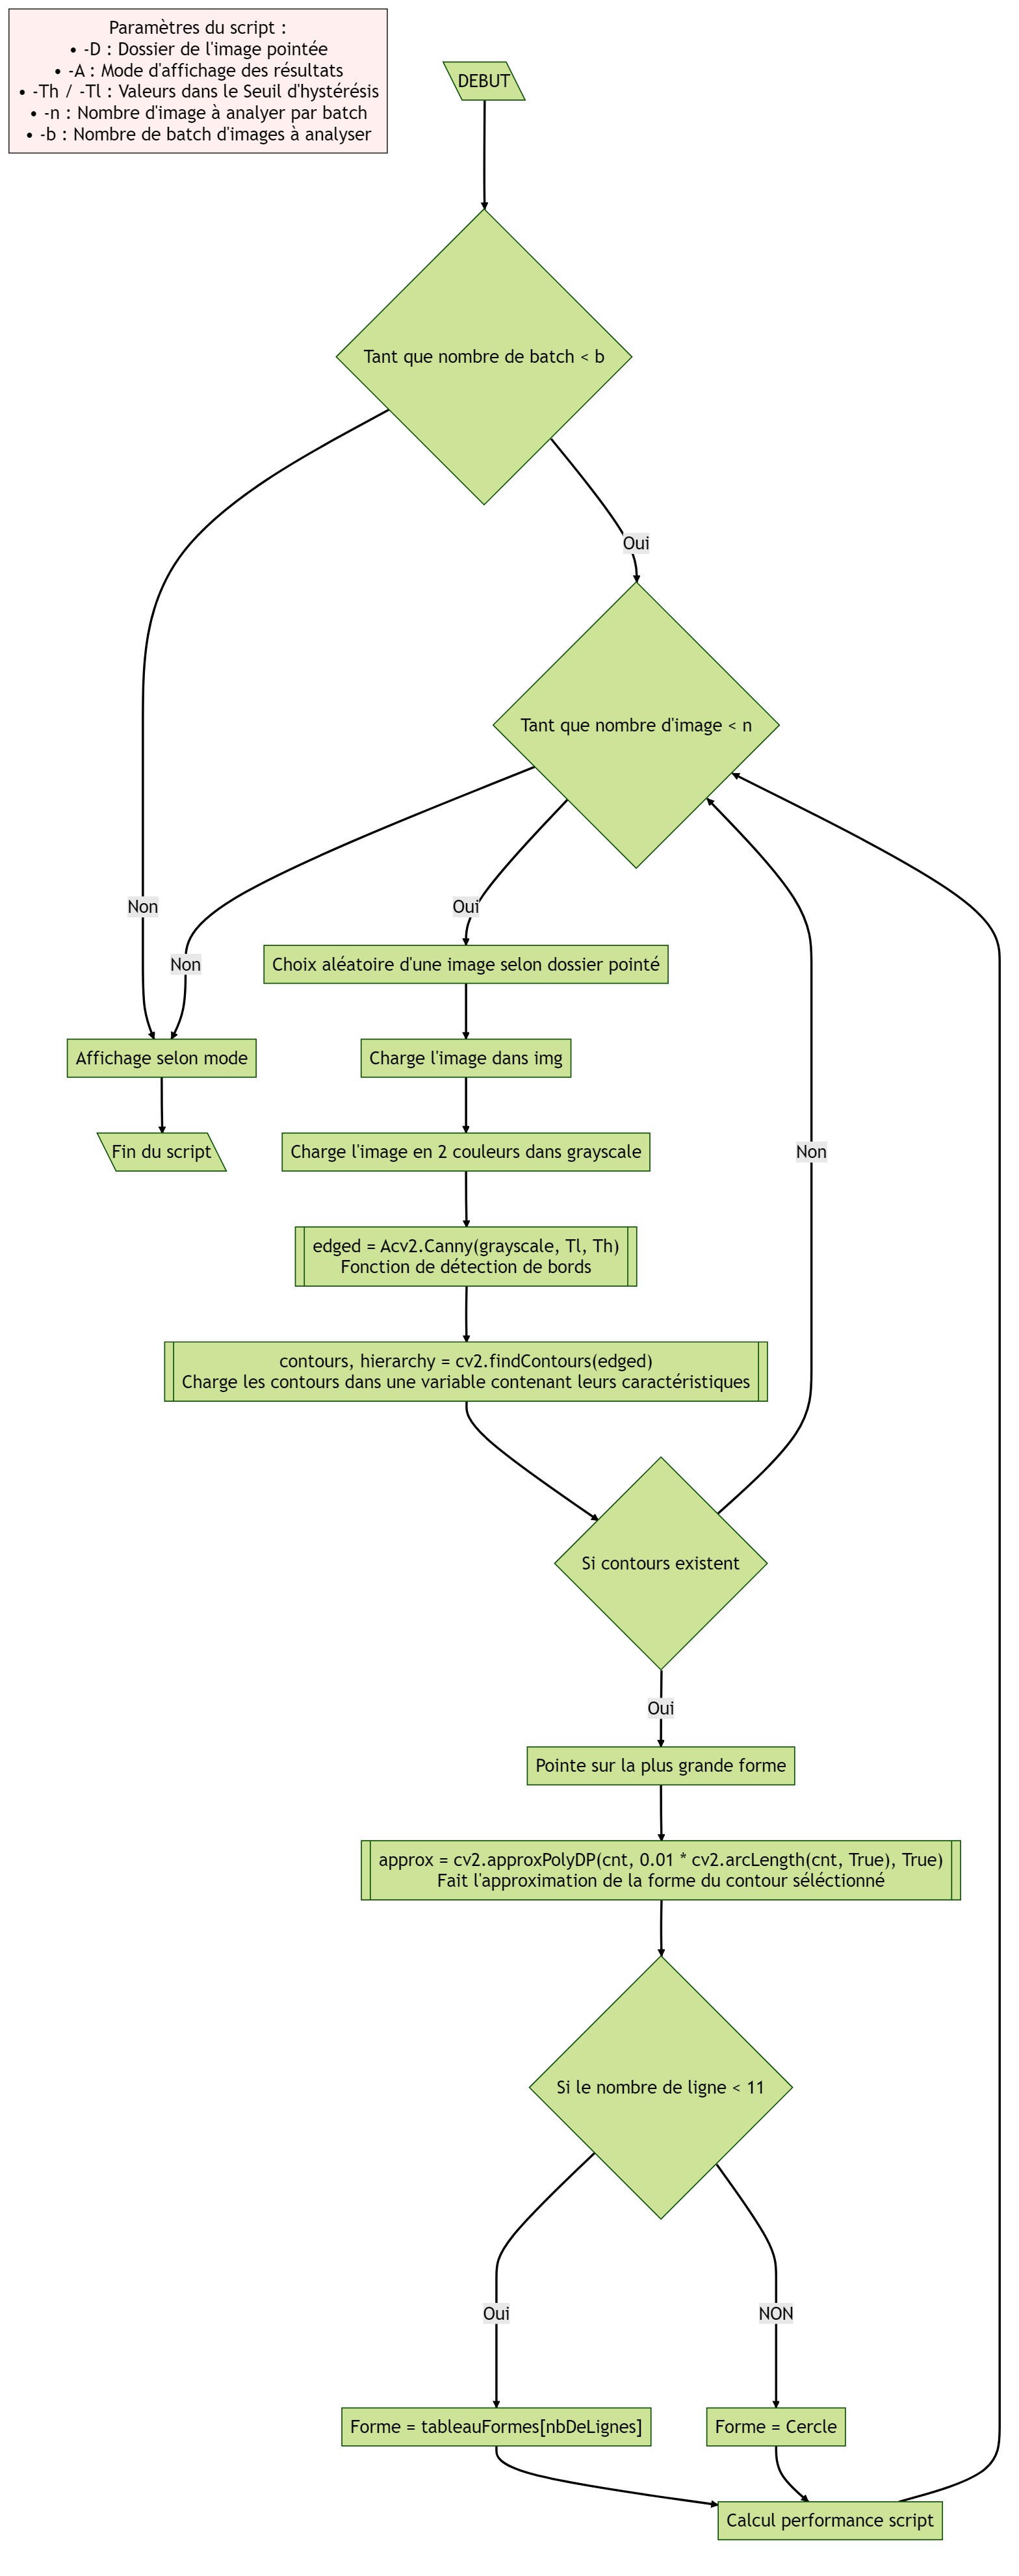
\includegraphics[height=1.2\textwidth]{../Flowcharts/ShapeDetect_B.png}
		\caption{Structogramme reconnaissance d'images}
		\label{fig:structo1}
	\end{figure}
	
	
	\subsubsection{Essais et étalonnage}
	Par la suite, j'ai pus obtenir des batteries d'analyses d'images comme sur la figure \ref{fig:batchexemple} avec des statistiques de réussites, ce qui m'a permis d'optimiser mes hyper-paramètres afin de calibrer mon algorithme.
	\begin{figure}[h]
		\centering
		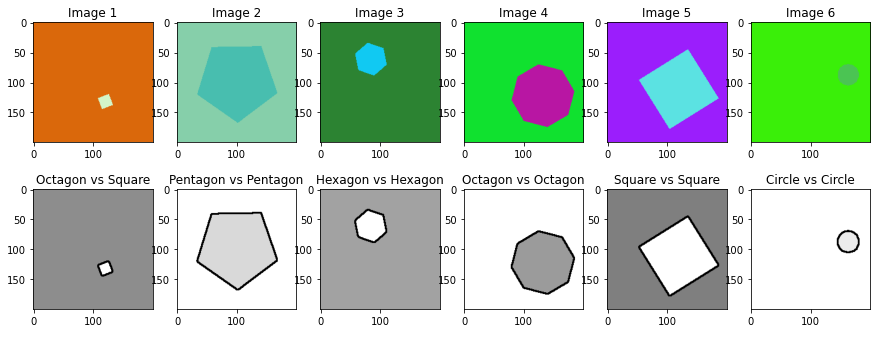
\includegraphics[width=\textwidth]{Figures/BatchExemple}
		\caption{Batch de 6 images}
		\label{fig:batchexemple}
	\end{figure}
	
	En sortie du script un pourcentage de réussite est donnée (voir figure \ref{fig:moyennebatchs}) où la moyenne des figures correspond à la moyenne des batchs.
	
	\begin{figure}[h]
		\centering
		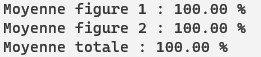
\includegraphics[width=0.5\linewidth]{Figures/MoyenneBatchs}
		\caption{Exemple de moyenne des batchs d'images}
		\label{fig:moyennebatchs}
	\end{figure}
	
	
	\paragraph{Description des paramètres : } Les paramètres principaux que j'ai fait varier sont les seuils d'hysteresis de la fonction canny d'openCV. Cette fonction est un filtrage qui capture les valeurs de bord qui fluctuent au-dessus et au-dessous des valeurs seuil \textbf{\textit{Tlow}} et \textbf{\textit{Thigh}}.
	
	\paragraph{Mesures : }
	\begin{center}
		\begin{tabular}{l l | l l}
			Réglage 1 & Réglage 2 & Mode Mesure & Moyenne de réussite \\
			\hline
			\textit{\textbf{Tlow}} = 10\quad\textit{\textbf{Thigh}} = 50 &  Convertis en B+W & 10img 10batchs & 51\%, 61.36\%, 70.75\% \\
			\textit{\textbf{Tlow}} = 10\quad\textit{\textbf{Thigh}} = 50 &  Convertis en B+W & 20img 20batchs & 62.42\% \\
			\textit{\textbf{Tlow}} = 10\quad\textit{\textbf{Thigh}} = 50 & Lis/charge en B+W & 20img 20batchs & 65.81\% \\
			\textit{\textbf{Tlow}} = 10\quad\textit{\textbf{Thigh}} = 30 & Lis/Charge en B+W & 20img 20batchs & 62.94\% \\
			\textit{\textbf{Tlow}} = 07\quad\textit{\textbf{Thigh}} = 45 & Lis/Charge en B+W & 20img 20batchs & 65\% \\
			\textit{\textbf{Tlow}} = 09\quad\textit{\textbf{Thigh}} = 45 & Lis/Charge en B+W & 20img 20batchs & 65.21\% \\
			\textit{\textbf{Tlow}} = 20\quad\textit{\textbf{Thigh}} = 40 & Lis/Charge en B+W & 20img 20batchs & 62.2\% \\
		\end{tabular}
	\end{center}
	
	Le réglage 2 est un test directement dans l'algorithme pour voir si il y avait une différence entre convertir l'image en 2 couleurs ou charger l'image en 2 couleurs, or il n'y a pas de différence visible dans les test.
	
	On peut voir que le taux de réussite n'est pas encore optimale mais ne descends presque jamais en dessous des 60\% sur une moyenne de 400 images ce qui me convient suffisamment pour continuer sur la suite du projet. J'ai décidé de conserver le mode \textit{\textbf{Tlow}} = 10 \textit{\textbf{Thigh}} = 50 avec \textit{Lis/charge en B+W} pour la version finale du script.

\subsection{Reconnaissance de formes - image réelles}
Afin d'atteindre l'objectif de reconnaissance d'images réelles, je m'y suis pris en deux parties avec deux scripts de complexités différents. L'un effectue une détection de forme et de contours sans déduire la forme, l'autre détecte les formes, tous les contours et déduit la forme de chacun des contours par une approximation en utilisant uniquement openCV.

	\subsubsection{Images utilisées}
	Pour tester mon algorithme, je n'ai pas utilisé des images optimale, sachant qu'une application industrielle impliquerait des images de meilleures qualité avec un éclairage adéquat, or j'ai utilisé mon téléphone et ai pris en photos des objet du quotidien.
	
	\paragraph{Problématique rencontrée : } Il est difficile d'optimiser un algorithme pour une détection de forme de pièces dont on ignore la nature, sachant que les images que j'ai utilisée sont détaillée et ont des ombres, beaucoup de contours sont détectés et filtrés ce qui rends parfois compliqué de définir quelle contour l'on souhaite décrire. La plupart du temps il s'agira du plus grand contour qui définira la forme de l'objet mais des erreurs peuvent avoir lieux. Si les seuils de détection des bords et les paramètres de la fonction qui les simplifie pour obtenir des formes moins complexes ne sont pas étalonnés pour des pièces spécifiques il es ardu de faire un script précis.
	
	\paragraph{Proposition de solution :} Pour un analyse d'image polyvalente et plus précise, l'on peut facilement implémenter sur python des modèles de machine learning entrainés sur de grandes quantités d'images. J'ai donc décidé d'également implémenter un script d'analyser d'image basé sur du machine learning plutôt que juste sur des fonction d'openCV\footnote{La libraire open-cv utilise également des modèles de machine learning}.
	
	\subsubsection{Explication du code}
	Je vais ici expliquer le modèle plus complet du script, sachant qu'il reprends les éléments des moins complexes (y-compris celui des dataset) ce qui permet de tous les expliquer par surcroit.
	
	\clearpage
	
	\begin{figure}[h!]
		\centering
		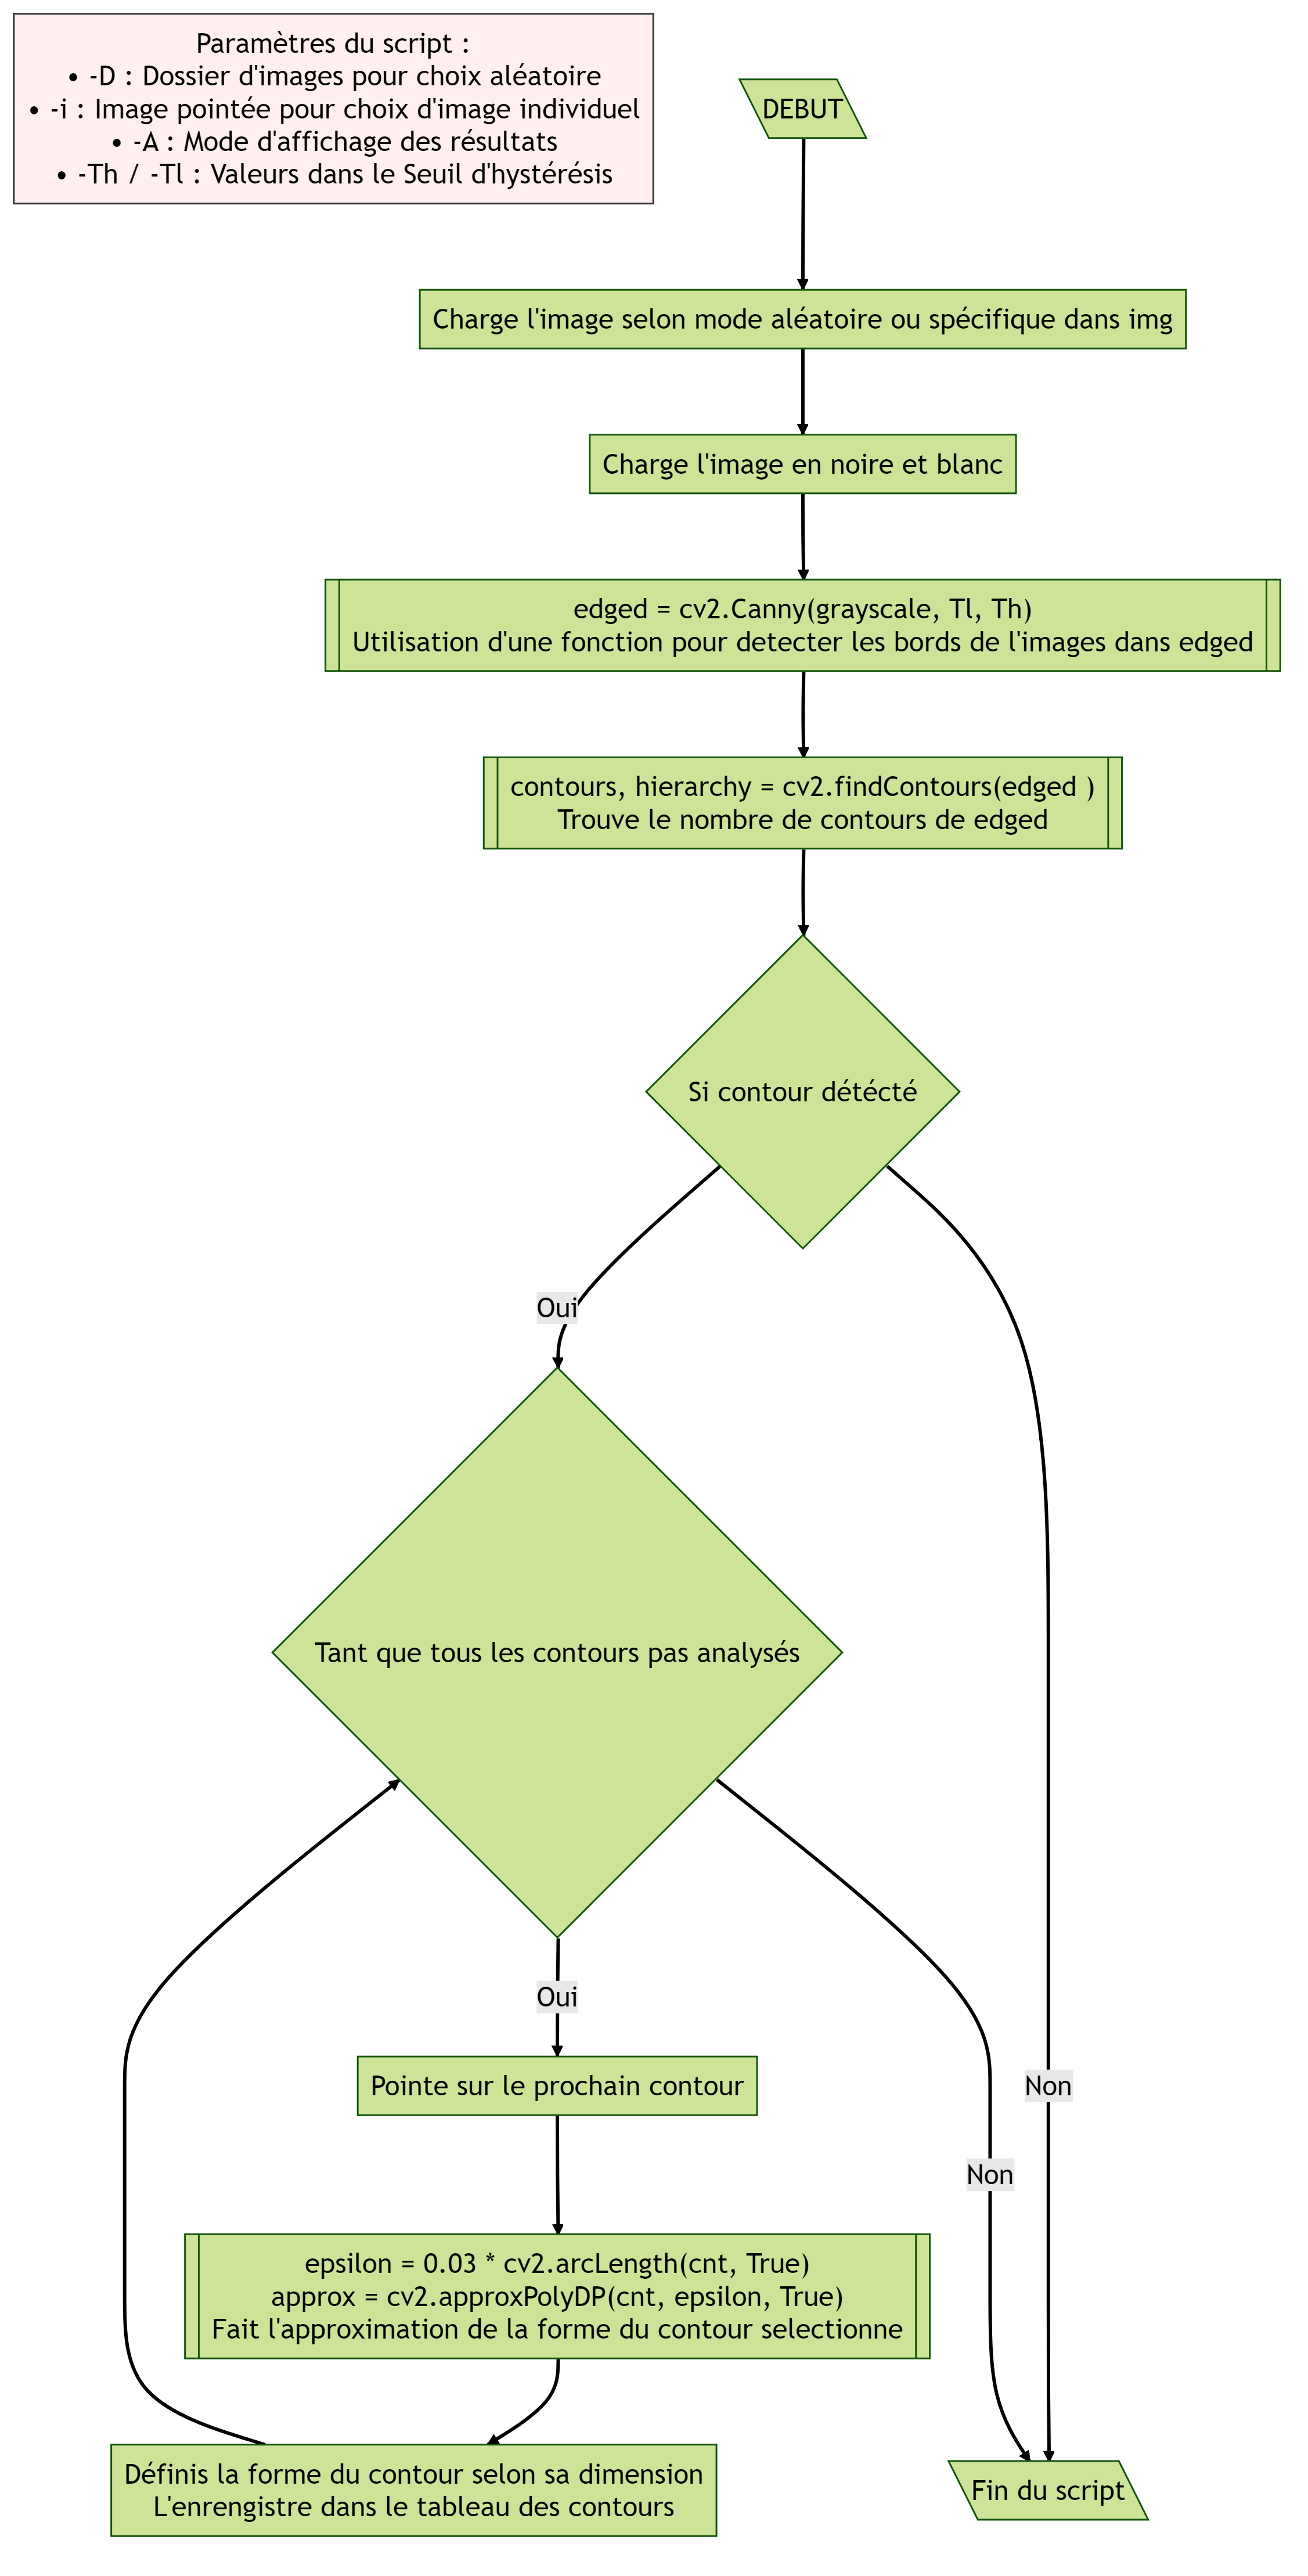
\includegraphics[width=0.65\linewidth]{../Flowcharts/ShapeRecogn.png}
		\caption{Flowchart du script ShapeRecognition-Approx}
		\label{fig:FlowShapeRecog}
	\end{figure}
	
	\clearpage
	
	
	\subsubsection{Résultats de l'algorithme}
	
	\begin{figure}[h]
		\centering
		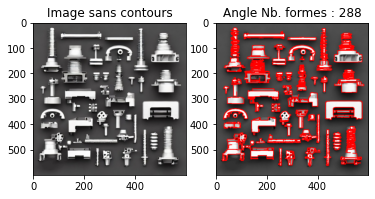
\includegraphics[width=0.8\linewidth]{Figures/ShapeRecogn_Exemple1}
		\caption{Essai de l'algorithme plusieurs pièces}
		\label{fig:shaperecognexemple1}
	\end{figure}
	
	\begin{figure}[h]
		\centering
		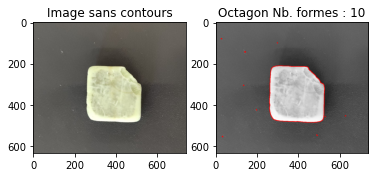
\includegraphics[width=0.8\linewidth]{Figures/ShapeRecogn_Exemple2}
		\caption{Essai de l'algorithme pièce unique}
		\label{fig:shaperecognexemple2}
	\end{figure}
	
	On peut constater que l'algorithme arrive à détecter les contours et à tenter de déduire leurs formes. Sur la figure \ref{fig:shaperecognexemple1} les \textit{288} contours détectés ont leurs formes déduite et enregistrées dans un tableau appelé \textit{shape}. Sur la figure \ref{fig:shaperecognexemple2} plusieurs contours sont détectés au-lieu d'un, ceci due à la mauvaise condition de l'image. La forme principale déduite est un octogone car le scripts détecte 8 lignes. Si l'on ajuste le scripte pour plus simplifier les contours, on arriverait à voir les 5 lignes principales qui constituent l'objet.

\clearpage	
\subsection{Description d'image - Machine learning}
J'ai donc décidé d'implémenter un script permettant d'exploiter un modèle de machine learning pour reconnaissance d'objets, il s'agit d'une approche finalement plus simple car sur python il est facile d'implémenter ce genre d'algorithme. Ce script permettra de compléter les lacunes des scripts précédents qui ne permettent pas de réellement décrire l'objet mais seulement des contours.

\subsubsection{Model utilisé}
Afin d'être facilement portable, il a fallut que je trouve un modèle léger mais suffisamment polyvalent, mon choix c'est donc porté sur \textit{resnet-18} ; Réseau neuronal résiduel sur 18 couches développé par microsoft qui prends $\sim 50MB$. Ce modèle est entrainé sur $11'689'512$ paramètres. Le modèle que j'ai utilisé est entrainé sur le dataset \textit{imagenet-1k} qui possède $1'281'167$ images d'entrainements.
Lien du modèle : \href{https://huggingface.co/microsoft/resnet-18}{https://huggingface.co/microsoft/resnet-18}. 

\subsubsection{Explication du code}

\begin{figure}[h]
	\centering
	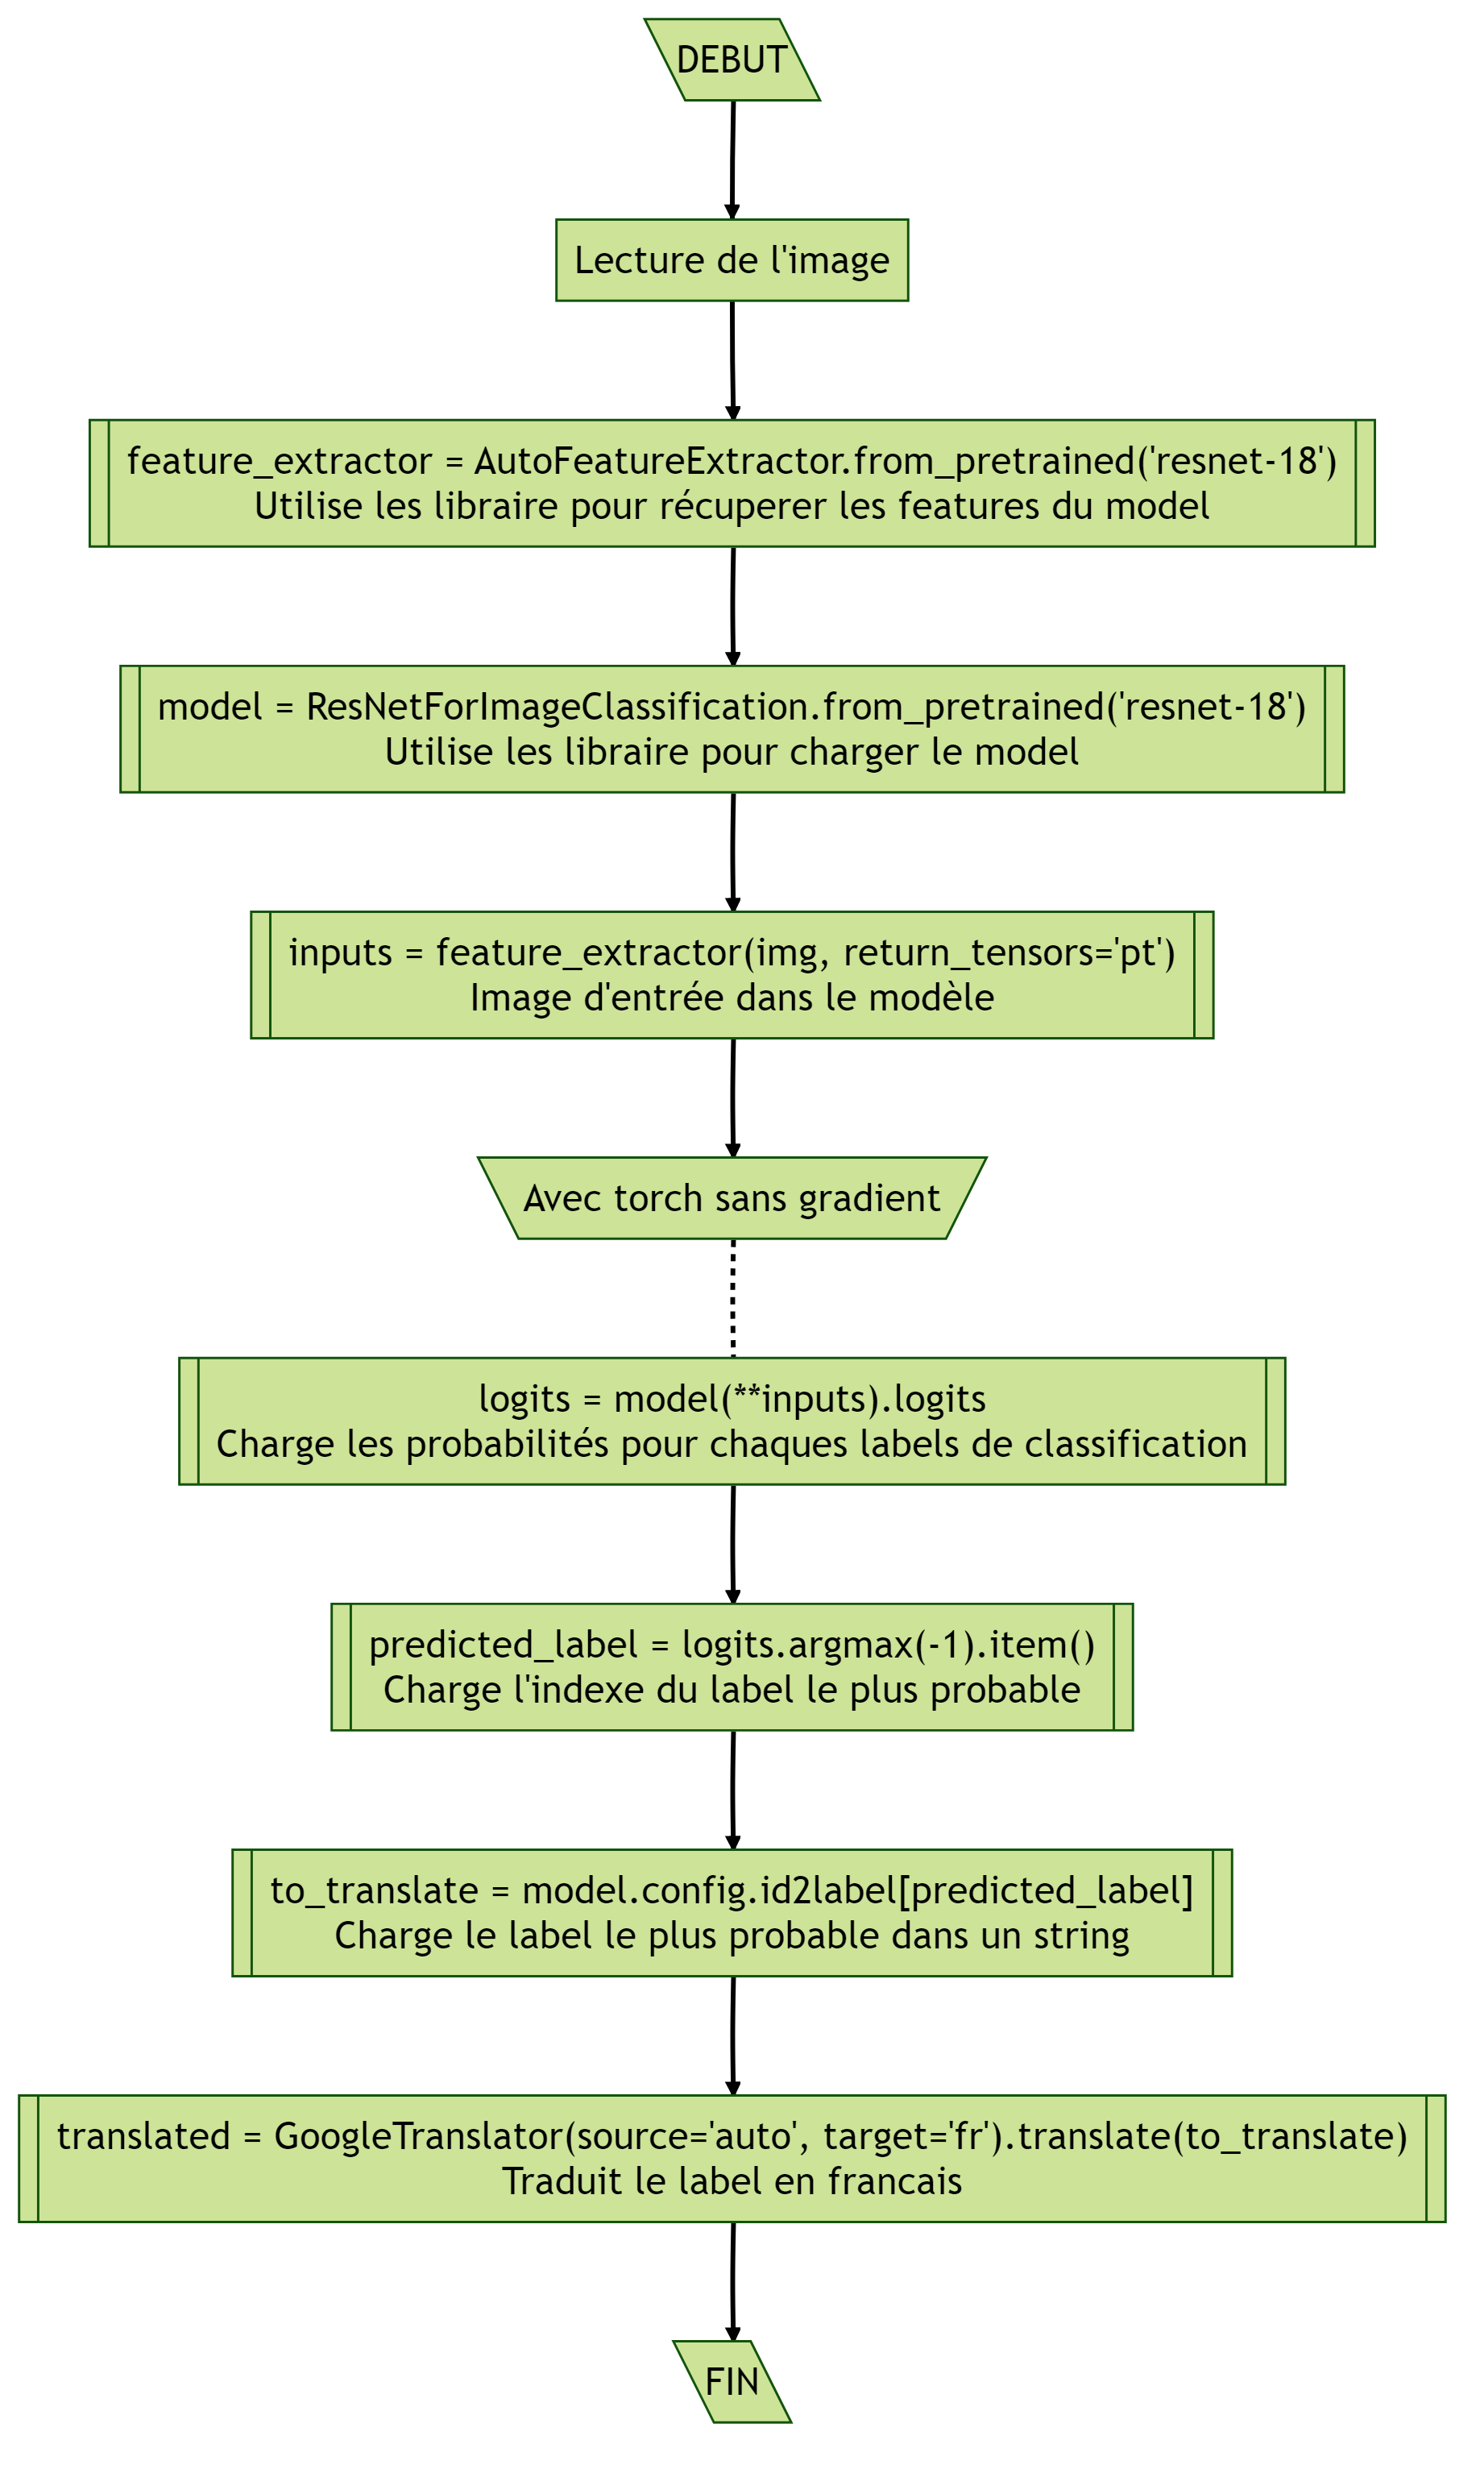
\includegraphics[width=0.483\linewidth]{../Flowcharts/img_descr.png}
	\caption{Flowchart du code - Machine learning}
	\label{fig:img_descr_flow}
\end{figure}


\clearpage	
\subsection{Application TKinter}
Afin de réunir tous les scripts j'ai décidé de développer une application avec une interface sur python, pour ce faire, j'ai utilisé le paquet \textit{PKinter} qui est une  bibliothèque graphique libre pour le langage Python, permettant la création d'interfaces graphiques. Faire une application graphique sur python simplifie également le déploiement sur raspberry.

\subsubsection{Fonctionnement}
TKinter permet d'utiliser des objet/widgets pour facilement mettre en place une interface graphique de façon très intuitive.

\begin{figure}[h]
	\centering
	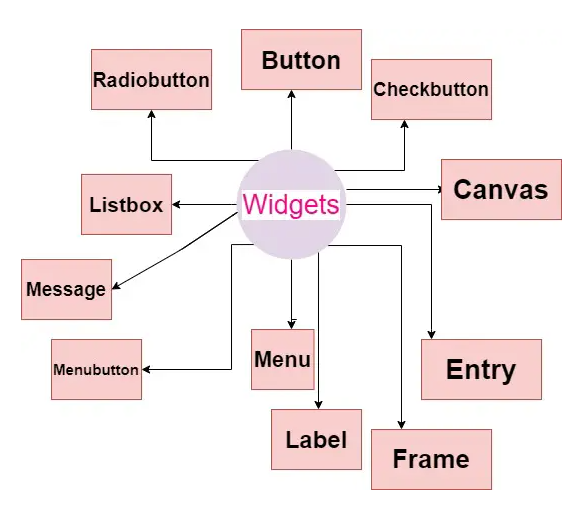
\includegraphics[width=0.5\linewidth]{Figures/TKinter_widgets}
	\caption{Widgets de TKinter}
	\label{fig:tkinterwidgets}
	\floatfoot{Source : \href{https://www.studytonight.com/tkinter/python-tkinter-widgets}{https://www.studytonight.com/tkinter/python-tkinter-widgets}}
\end{figure}


\paragraph{Implémentation des scripts :} Afin de réutiliser les algorithmes précédents j'ai dû les convertir en fonction avec paramètres et retours, puis de les \textit{importer} dans l'application graphique.

\begin{figure}[h]
	\centering
	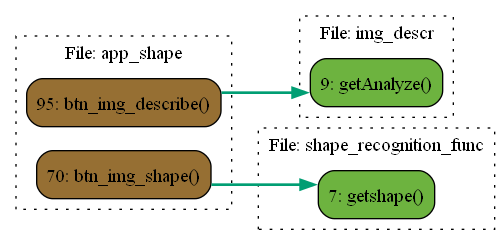
\includegraphics[width=0.56\linewidth]{Figures/flowchart-fichiers}
	\caption{Inclusion des différents fichier dans l'application}
	\label{fig:flowchart-fichiers}
\end{figure}


\clearpage
\subsubsection{Démonstration}

\begin{figure}[h]
	\centering
	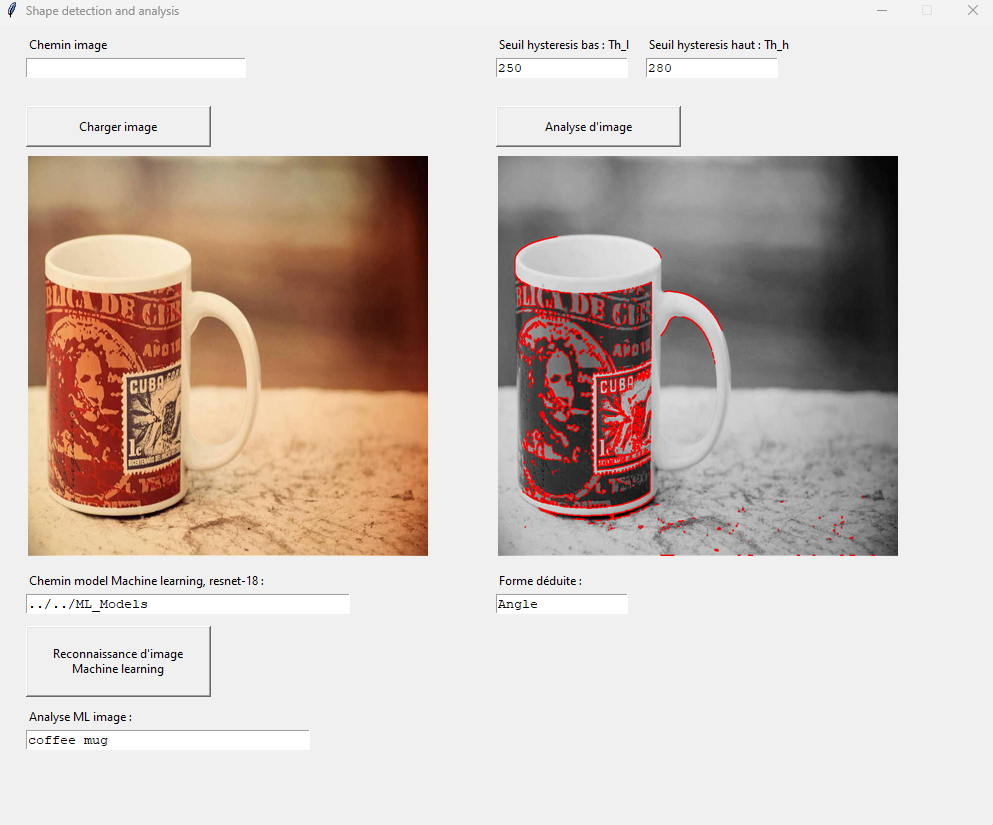
\includegraphics[width=0.8\linewidth]{Figures/Exemple_appli}
	\caption{Application graphique}
	\label{fig:exempleappli}
\end{figure}

En colant une image locale dans "\textit{Chemin image}" puis en la chargeant, on peut la visualiser sans analyse. Ensuite en réglant les seuils de détections, on peut lancer l'algorithme d'analyser des contours et de déduction de forme (A droite de la figure \ref{fig:exempleappli}). Enfin, en appuyant sur "\textit{Reconnaissance d'image Machine learning}" on peut lancer l'analyse du modèle ResNet18 afin de décrire l'image. 

\paragraph{Implémentation pour webcam :} Lire le flux vidéo d'une webcam est similaire à charge une image via un lien, il serait facile de modifier l'application pour permettre de lire une image par un flux vidéo. L'application serait plus utile en temps-réelle il serait donc préférable de la modifier ou d'en faire une nouvelle à l'avenir. Ici il s'agit surtout de regrouper les 2 algorithmes précédents dans une application afin de facilement les tester, pour les perfectionner.

%---
\clearpage
\section{Conclusion}

Dans ce projet de programmation orientée objet, j'ai eu l'occasion de :
\begin{itemizeFB}
	\item[$\bullet$]  Développer des scripts permettant d'extraire et d'analyser des contours d'images.
	\item[$\bullet$] Mettre en place et tester des algorithme sur des images réelle ou issues de dataset.
	\item[$\bullet$] Implémenter un modèle de machine learning pour de la reconnaissance d'image.
	\item[$\bullet$] Développer une application python regroupant les scripts principaux issus de ce travail.
\end{itemizeFB}

J'ai pu, perfectionner mes connaissances sur le language python ainsi que pu apprendre de nombreuses choses sur le traitement de l'image et la machine vision. J'ai trouvé ce travail très intéressant et diversifié, la liberté quant aux directions du projet était très agréable.

\paragraph{Perspective du projet :} Je n'ai pas eu l'occasion d'implémenter les algorithme sur un raspberry. Pour le faire, il faudrait bien configurer l'interpréteur python avec la bonne version selon les paquets utilisés, le tout par la distribution Anaconda. Il faudrait également selon la webcam utilisée mettre en place la lecture de celle-ci et adapter les scripts existant pour lire ce flux plutôt que des images fixes.

\vspace{120mm}
\begin{tabular}{@{}p{0.4\textwidth}p{0.1\textwidth}p{0.4\textwidth}@{}}
	
	\hrulefill && \\
	Ali Zoubir && \\
	ETML-ES - Génie électrique \\
	Lausanne, le \today \\
\end{tabular}

